\documentclass[11pt,fleqn,dvipsnames,usenames]{article}

% to keep this file less overwhelming
% packages to include

\usepackage[dvipsnames, table]{xcolor}

\usepackage{
  amsmath,
  amssymb, 
  arydshln, % for hyphenated lines in block matrices
  fancyhdr, % needed for header at top of each page
  graphicx, % to include pictures
  hyperref, % for hyper links
  mathtools, % for a longer arrow
  multicol, % displaying enumerates and itemizes into multiple columns
  multirow, % for tables
  multido, % for TOC
  pgfplots, % for axis environment within tikz pictures
  systeme,
  tikz,
}

\usepackage[inline, shortlabels]{enumitem}


% global constants
\newcommand{\term}{Fall 2024}
\newcommand{\course}{Math 2210}

% mathbb aliases
\newcommand{\COMPLEX}{\mathbb{C}}
\newcommand{\C}{\COMPLEX}
\newcommand{\REAL}{\mathbb{R}}
\newcommand{\R}{\REAL}
\newcommand{\RATIONAL}{\mathbb{Q}}
\newcommand{\Q}{\RATIONAL}
\newcommand{\INTEGER}{\mathbb{Z}}
\newcommand{\Z}{\INTEGER}
\newcommand{\ZN}{\INTEGER_{n}}
\newcommand{\NATURAL}{\mathbb{N}}
\newcommand{\N}{\NATURAL}

\newcommand{\ZX}{\Z[x]}
\newcommand{\ZNX}{\ZN[x]}
\newcommand{\QX}{\Q[x]}
\newcommand{\RX}{\R[x]}
\newcommand{\CX}{\C[x]}
\newcommand{\CZ}{\C[z]}

% complex number aliases
\newcommand{\RE}[1]{\text{Re}\left(#1\right)}
\newcommand{\IM}[1]{\text{Im}\left(#1\right)}
\newcommand{\CC}[1]{\overline{#1}}
\newcommand{\ARG}[1]{\text{arg}\left(#1\right)}
\newcommand{\PARG}[1]{\text{Arg}\left(#1\right)}

% for financial stuff
\newcommand{\dollar}{\mathrm{\$}}

% nicer looking trig functions
\newcommand{\SIN}[1]{\sin\left(#1\right)}
\newcommand{\COS}[1]{\cos\left(#1\right)}
\newcommand{\TAN}[1]{\tan\left(#1\right)}
\newcommand{\CSC}[1]{\csc\left(#1\right)}
\newcommand{\SEC}[1]{\sec\left(#1\right)}
\newcommand{\COT}[1]{\cot\left(#1\right)}

% number theory
\newcommand{\ndiv}{|\kern-0.9ex{/}}

% automatically resize set brackets
\newcommand{\SET}[1]{\left\{#1\right\}}

% sums and products
\newcommand{\SUM}{\displaystyle\sum\limits}
\newcommand{\PROD}{\displaystyle\prod\limits}
\newcommand{\LIMIT}{\displaystyle\lim\limits}
\newcommand{\of}{\circ}
\newcommand{\restrict}[1]{\raisebox{-.5ex}{$|$}_{#1}}

% set intersection and union
\newcommand{\CAP}{\displaystyle\bigcap\limits}
\newcommand{\CUP}{\displaystyle\bigcup\limits}

% polynomials
\newcommand{\DEG}[1]{\ensuremath{\text{deg}\left(#1\right)}}

% max and min
\newcommand{\MAX}[1]{\ensuremath{\max\left\{#1\right\}}}
\newcommand{\MIN}[1]{\ensuremath{\min\left\{#1\right\}}}

% gcd and lcm
\newcommand{\GCD}[1]{\ensuremath{\text{gcd}\left(#1\right)}}
\newcommand{\LCM}[1]{\ensuremath{\text{lcm}\left(#1\right)}}

% for writing logic within mathematics environment
\newcommand{\FORALL}{\ensuremath{\text{ for all }}}
\newcommand{\FORSOME}{\ensuremath{\text{ for some }}}

% matrix notation
\newcommand{\MATRIX}[2]{\ensuremath{\left[\begin{array}{#1}#2\end{array}\right]}}
\newcommand{\COLUMN}[1]{\ensuremath{\left[\begin{array}{r}#1\end{array}\right]}}
\newcommand{\BY}{\times}

% vector notation
%\newcommand{\vv}{\overset{\rightharpoonup}}
\newcommand{\vv}[1]{{\bf #1}}
\newcommand{\arr}{\overrightarrow}

% dot product
\newcommand{\dotp}{{\scriptstyle\bullet}}

% Text macros
\newcommand{\KER}[1]{\ensuremath{\text{ker}\left(#1\right)}}
\newcommand{\IMG}[1]{\ensuremath{\text{im}\left(#1\right)}}
\newcommand{\CHAR}[1]{\ensuremath{\text{char}\left(#1\right)}}
\newcommand{\BIGO}[1]{\ensuremath{\mathcal{O}\left(#1\right)}}
\newcommand{\TR}[1]{\ensuremath{\text{tr}\left(#1\right)}}

% abbreviations
\newcommand{\ds}{\displaystyle}
\newcommand{\md}{\mdseries}

% abbreviations for vertical/horizontal spaces
\newcommand{\vsp}{\vspace{0.5cm}}
\newcommand{\smsp}{\vspace{0.25cm}} % small space
\newcommand{\vsmsp}{\vspace{0.1cm}} % very small space
\newcommand{\hsp}{\hspace{0.25cm}}

% new operators
\DeclareMathOperator\SPAN{Span}
\newcommand{\SPANOF}[1]{\ensuremath{\SPAN\left\{#1\right\}}}
\DeclareMathOperator\PROJ{proj}
\DeclareMathOperator\PERP{perp}

% underlining definitions
\newcommand{\DEF}[1]{\textbf{\ul{#1}}}

% environments
\newtheorem{theorem}{Theorem}[subsection]
\newtheorem*{theorem*}{Theorem}
\newtheorem{corollary}[theorem]{Corollary}
\newtheorem*{corollary*}{Corollary}
\newtheorem{lemma}[theorem]{Lemma}

\theoremstyle{definition}
\newtheorem{definition}[theorem]{Definition}
\newtheorem*{definition*}{Definition}
\newtheorem{example}[theorem]{Example}
\newtheorem*{example*}{Example}
\newtheorem{examples}[theorem]{Examples}
\newtheorem*{examples*}{Examples}
\newtheorem{exercise}[theorem]{Exercise}
\newtheorem*{exercise*}{Exercise}
\newtheorem{exercises}[theorem]{Exercises}
\newtheorem{remark}[theorem]{Remark}
\newtheorem{remarks}[theorem]{Remarks}

% make proof boxes solid
\renewcommand{\qedsymbol}{$\blacksquare$}

% quick abbreviations to avoid using latex environments (gradually phasing these out)
\newcommand{\analogy}{\noindent \textbf{Analogy:} }
\newcommand{\answer}{\noindent \textbf{Answer:} }
\newcommand{\answers}{\noindent \textbf{Answers:} }
\newcommand{\application}{\noindent \textbf{Application:} }
\newcommand{\background}{\noindent \textbf{Background:} }
\newcommand{\caution}{\noindent \textbf{Caution:} }
\newcommand{\conclusion}{\noindent \textbf{Conclusion:} }
\newcommand{\consequence}{\noindent \textbf{Consequence:} }
\newcommand{\convention}{\noindent \textbf{Convention:} }
\newcommand{\conventions}{\noindent \textbf{Conventions:} }
\newcommand{\crlry}{\noindent \textbf{Corollary:} }
\newcommand{\defn}{\noindent \textbf{Definition:} }
\newcommand{\details}{\noindent \textbf{Details:} }
\newcommand{\nexamples}[1]{\noindent \textbf{Examples (#1):}} 
\newcommand{\exception}{\noindent \textbf{Exception:} }
\newcommand{\nexercise}[1]{\noindent \textbf{Exercise (#1):}} 
\newcommand{\nexercises}[1]{\noindent \textbf{Exercises (#1):}} 
\newcommand{\fact}{\noindent \textbf{Fact:} }
\newcommand{\facts}{\noindent \textbf{Facts:} }
\newcommand{\fix}{\noindent \textbf{Fix:} }
\newcommand{\formula}{\noindent \textbf{Formula:} }
\newcommand{\goal}{\noindent \textbf{Goal:} }
\newcommand{\goals}{\noindent \textbf{Goals:} }
\newcommand{\hint}{\noindent \textbf{Hint:} }
\newcommand{\idea}{\noindent \textbf{Idea:} }
\newcommand{\illustration}{\noindent \textbf{Illustration:} }
\newcommand{\important}{\noindent \textbf{Important:} }
\newcommand{\lema}{\noindent \textbf{Lemma:} }
\newcommand{\midea}{\noindent \textbf{Main Idea:} }
\newcommand{\motivation}{\noindent \textbf{Motivation:} }
\newcommand{\nthm}[1]{\noindent \textbf{Theorem} (\textit{#1}):}
\newcommand{\notation}{\noindent \textbf{Notation:} }
\newcommand{\note}{\noindent \textbf{Note:} }
\newcommand{\notes}{\noindent \textbf{Notes:} }
\newcommand{\observation}{\noindent \textbf{Observation:} }
\newcommand{\observations}{\noindent \textbf{Observations:} }
\newcommand{\pict}{\noindent \textbf{Picture:} }
\newcommand{\plan}{\noindent \textbf{Plan:} }
\newcommand{\prf}{\noindent \textbf{Proof:} }
\newcommand{\problem}{\noindent \textbf{Problem:} }
\newcommand{\properties}{\noindent \textbf{Properties:} }
\newcommand{\question}{\noindent \textbf{Question:} }
\newcommand{\questions}{\noindent \textbf{Questions:} }
\newcommand{\recall}{\noindent \textbf{Recall:} }
\newcommand{\reason}{\noindent \textbf{Reason:} }
\newcommand{\reminder}{\noindent \textbf{Reminder:} }
\newcommand{\solution}{\noindent \textbf{Solution:} }
\newcommand{\nsolution}[1]{\noindent \textbf{Solution #1:} }
\newcommand{\setting}{\noindent \textbf{Setting:} }
\newcommand{\strategy}{\noindent \textbf{Strategy:} }
\newcommand{\summary}{\noindent \textbf{Summary:} }
\newcommand{\terminology}{\noindent \textbf{Terminology:} }
\newcommand{\thm}{\noindent \textbf{Theorem:} }
\newcommand{\work}{\noindent \textbf{Work:} }

% gray line across pagewidth
\newcommand{\GRAYLINE}{
  {\color{gray}\leaders\vrule width \textwidth\vskip0.4pt} % or other desired thickness
  \vskip\medskipamount % ditto
  \nointerlineskip
  \smsp
}

% Where to look for pngs and jpegs
\graphicspath{{Images//}}

\usepackage[includehead, includefoot, left= 2cm, top =1.5cm, bottom = 1.5cm, textwidth=17.5cm]{geometry}

\usepackage{pifont, amsmath}

\pagestyle{fancy}
\fancyhf{}
\renewcommand{\headrulewidth}{1pt}
%\fancyhead[R]{\bfseries\sffamily\thepage}
%\fancyfoot[C]{\bfseries\sffamily\thepage}
\fancyhead[L]{\nouppercase{\bfseries\sffamily\leftmark}}

% used when adding fill-in-the-blanks for students
\newcommand{\blank}[1]{\underline{\hspace{#1}}}

% indents annoy me, and so does repeatedly typing \noindent
\newcommand{\p}{\noindent}
\newcommand{\ENDPRF}{\hfill $\blacksquare$}

\begin{document}

\fancyhead[L]{Math 2210}
\fancyhead[C]{
\includegraphics[width=5cm, trim= 0 0.4cm 0 0]{TRU_logo}}
\fancyhead[R]{\term}
\renewcommand{\headrulewidth}{0.4pt}

\setulcolor{red}

\setcounter{section}{0}
\section{Arithmetic in \texorpdfstring{$\INTEGER, \RATIONAL, \REAL$}{Z, Q, R} and \texorpdfstring{$\COMPLEX$}{C}}
\setcounter{subsection}{0}


\subsection{The Division Algorithm}

The set of \DEF{natural numbers} is written as
\begin{center}
$\NATURAL = \SET{1,2,3,\dots}$
\end{center}
and the set of \DEF{integers} is written as
\begin{center}
\item $\INTEGER = \SET{0, \pm 1, \pm 2,\pm 3,\dots}$
\end{center}
\vsp

\p New sets may be introduced using set-builder notation, for example:
\begin{center}
$S = \SET{n\in\INTEGER:n\geq 0}$
\end{center}
represents the set of all positive integers.
\vsp

\begin{theorem}[The Division Algorithm] Let $a,b > 0$ be integers.  There exists unique $q,r\in\INTEGER$ such that
\begin{center}
$a = bq + r$ and $0\leq r < b$.
\end{center}
\end{theorem}

\begin{proof}

(Existence) If $a < b$, then the conclusion holds with $q = 0$ and $r = a$.  Otherwise, there exists $q\in\INTEGER$ such that $bq \leq a < b(q + 1)$.  In this case the conclusion holds with $r = a - bq$.
\vsp

\p (Uniqueness) Now suppose that $q, q', r, r'\in \INTEGER$ such that
\begin{center}
$a = bq + r$ and $a = bq' + r'$.
\end{center}
By rearranging, we obtain $r - r' = b(q' - q)$.  Since $0 \leq r < b$ and $0 \leq r' < b$, we obtain
\begin{center}
$-b < r - r' < b$,
\end{center}
or
\begin{center}
$-b < b(q' - q) < b$,
\end{center}
which implies
\begin{center}
$-1 < q' - q < 1$,
\end{center}
which forces $q = q'$.  It immediately follows that $r = r'$.
\end{proof}
\newpage

\begin{corollary} Let $a > 0$ and $b$ be integers with $b\neq 0$.  There exists unique $q,r\in\INTEGER$ such that $a = bq + r$ and $0\leq r < |b|$.
\end{corollary}

\begin{proof} By the Division algorithm, there exists unique $q,r\in \INTEGER$ such that
\begin{center}
$a = (-b)q + r$ and $0 \leq r < -b$.  
\end{center}
It follows that $a = b(-q) + r$ and $0\leq r < |b|$, which establishes existence.  Uniqueness is left as an exercise.
\end{proof}

\subsection{Divisibility}

\begin{definition} Let $a,b\in\INTEGER$ and $b\neq 0$.  We say that $b$ \DEF{divides} $a$ (or that $b$ is a \DEF{divisor} of $a$) if there exists $k\in\INTEGER$ such that $a = kb$.
\end{definition}

\notation If $b$ divides $a$, we write $b | a$.  Otherwise we write $b\ndiv a$.
\vsp

\examples
\begin{enumerate}[(a)]
\item $6 | 24$ because $24 = 4\cdot 6$
\item $5\ndiv 24$
\item $-4 | 36$ because $36 = (-9)(-4)$
\item Every non-zero $b\in\INTEGER$ divides $0$ because $0 = 0\cdot b$.
\item $1$ is a divisor of every $a\in\INTEGER$ because $a = a\cdot 1$.
\end{enumerate}

\begin{exercise} Prove the following.
\begin{enumerate}[(a)]
\item If $b|a$ then $-b|a$.
\item If $b|a$ then $b|-a$.
\item If $b|a$ then $-b|-a$.
\item If $b|a$ then $b$ divides $|a|$.
\end{enumerate}
\end{exercise}

\begin{remark}
If $a\neq 0$ and $b|a$, then $a = bc$ for some $c\in\INTEGER$, and hence $|a| = |b|\cdot |c|$.  Since $|c|\geq 1$, we must have $|b|\leq |a|$, so there are only finitely many divisors of $a$.
\end{remark}

\begin{example}
The divisors of $18$ are $\pm1, \pm2,\pm3,\pm6,\pm18$.
\end{example}

\exercises
\begin{enumerate}
\item Prove the following.
\begin{enumerate}[(a)]
\item If $b|a$, then $b|ac$ for any $c\in\INTEGER$.
\item If $b|a$ and $b|c$, then $b|a+c$.
\item If $b|a$ and $b|c$, then $b|sa+tc$ for any $s,t\in\INTEGER$.
\item If $b|a$ then $b^2|a^2$.
\end{enumerate}
\item If $b|ac$, does it necessarily follow that $b|a$ or $b|c$?
\item If $b|a+c$, does it necessarily follow that $b|a$ or $b|c$? 
\end{enumerate}

\begin{example}
Use the Division Algorithm to prove that the square of any integer $a$ is of the form $3k$ or $3k+1$ for some $k\in\INTEGER$.
\end{example}

\solution If $a$ is divisible by $3$, then $a = 3k$ for some $k\in\INTEGER$.  Hence $a^2 = (3k)^2 = 9k^2 =  3\cdot (3k^2)$.
\vsp

\p Hence it suffices to show that if $3\ndiv a$, then $a^2 = 3k +1$ for some $k\in\INTEGER$.
\vsp

\p Assume that $3\ndiv a$, and use the Division Algorithm to choose $q,r\in\INTEGER$ satisfying
\begin{center}
$a^2 = 3q + r$ and $0 \leq r < 3$.
\end{center}
\p By assumption, we must have $r=1$ or $r=2$.  If $r = 1$, then $a^2 = (3k+1)^2 = 9k^2 + 6k + 1 = 3(3k^2 + 2k) + 1$.  If $r = 2$, then $a^2 = (3k+2)^2 = 9k^2 + 12k + 4 = 3(3k^2 + 4k + 1) + 1$. \ENDPRF
\vsp

\begin{exercise}
Prove that the cube of any integer $a$ is of the form $9k, 9k+1$, or $9k+8$ for some $k\in\INTEGER$.
\end{exercise}

\defn The \DEF{greatest common divisor} of $a,b\in\INTEGER$ is the largest of all integers which divide both $a$ and $b$.  In other words, $d\in\INTEGER$ is the greatest common divisor of $a$ and $b$ if:
\begin{enumerate}[(1)]
\item $d$ is a common divisor of both $a$ and $b$.
\item If $d'$ is also a common divisor of both $a$ and $b$, then $d'\leq d$.
\end{enumerate}
\vsp

\notation The greatest common divisor of $a,b\in\INTEGER$ is denoted by $\GCD{a,b}$.
\vsp

\begin{example}
Find $\GCD{210,39}$.
\end{example}

\solution The divisors of $210$ are
\begin{center}
$1,2,3,5,6,7,10, 14, 15, 21, 30, 35, 42, 70, 105$, and $210$.
\end{center}
The divisors of $39$ are
\begin{center}
$1,3,13$, and $39$.
\end{center}
\p The largest number which appears in both lists is $3$.  Hence $\GCD{210,39} = 3$.
\vsp

\begin{example}
For any positive $a\in\INTEGER$, $\GCD{a,0} = 0$.  Certainly $a$ is a common divisor of $a$ and $0$, and there cannot be any larger one since if $b|a$ then $0\leq b\leq a$.
\end{example}

\note For any $b\in\INTEGER$, both $b$ and $-b$ have the same divisors.  Hence
\begin{center}
$\GCD{a,b} = \GCD{-a,b} = \GCD{a,-b} = \GCD{-a,-b}$
\end{center}
\vsp

\nthm{Euclidean Algorithm} Let $a,b\in\INTEGER$ be positive.  If $b|a$ then $\GCD{a,b} = b$.  If $b\ndiv a$, then apply the Division Algorithm repeatedly as follows.

\begin{itemize}[\ ]
\item $a = q_{0}b + r_{0}$ for some $q_{0},r_{0}\in\INTEGER$ with $0 \leq r_{0} < b$.
\item $b = q_{1}r_{0} + r_{1}$ for some $q_{1},r_{1}\in\INTEGER$ with $0 \leq r_{1} < r_{0}$.
\item $r_{0} = q_{2}r_{1} + r_{2}$ for some $q_{2},r_{2}\in\INTEGER$ with $0 \leq r_{2} < r_{1}$.
\item $r_{1} = q_{3}r_{2} + r_{3}$ for some $q_{3},r_{3}\in\INTEGER$ with $0 \leq r_{3} < r_{2}$.
\item \phantom{$r_{0} = q_{2}r_{1} + r_{2}$ for some}$\vdots$
\item $r_{t-2} = q_{t}r_{t-1} + r_{t}$ for some $q_{t},r_{t}\in\INTEGER$ with $0 \leq r_{t} < r_{t-1}$.
\item $r_{t-1} = q_{t+1}r_{t} + 0$ for some $q_{t+1}\in\INTEGER$,
\end{itemize}
with the process terminating on the $(t+2)$-nd iteration, where $r_{t}$ divides $r_{t-1}$.  In this case, the final non-zero remainder is the greatest common divisor of $a$ and $b$.  That is, $\GCD{a,b} = r_{t}$.
\vsp

\p The following consequence of the Euclidean Algorithm is known as B\'{e}zout's Identity.  Its proof consists  essentially of applying the Euclidean Algorithm in reverse.
\vsp

\crlry Let $a,b\in\INTEGER$ be positive.  There exists $s,t\in\INTEGER$ such that $\GCD{a,b} = sa + tb$.
\vsp

\begin{example}
$\GCD{84,60} = 12$, since
\begin{itemize}[\ ]
\item $84 = 1\cdot 60 + 24$
\item $60 = 2\cdot 24 + 12$
\item $24 = 2\cdot 12 + 0$
\end{itemize}

\p Moreover, we may use these equations to write $12 = 60 - 2\cdot 24 = 60 - 2\cdot (84 - 60) = -2\cdot 84 + 3\cdot 60$.
\end{example}

\begin{example}
$\GCD{324, 148} = 4$, since
\begin{itemize}[\ ]
\item $324 = 2\cdot 148 + 28$
\item $148 = 5\cdot 28 + 8$
\item $28 = 3\cdot 8 + 4$
\item $8 = 2\cdot 4 + 0$
\end{itemize}

\p Moreover, we may use these equations to write
\begin{center}
$4 = 28 - 3\cdot 8 = 28 - 3\cdot (148 - 5\cdot 28) = -3\cdot 148 + 16\cdot 28 = -3\cdot 148 + 16\cdot (324 - 2\cdot 148) = 16\cdot 324 - 35\cdot 148$.
\end{center}
\end{example}
\newpage

\caution This is not to be misinterpreted.  Simply observing $d = sa + tb$ for some $s,t\in\INTEGER$ is not sufficient to conclude that $d = \GCD{a, b}$!  For example,
\begin{center}
$12 = (-1)\cdot 88 + 100$,
\end{center}
but $12$ is not a divisor of $88$ and hence cannot be equal to $\GCD{88,100}$.
\vsp

\begin{exercise}
If $n\in\INTEGER$, what are the possible values for
\begin{enumerate}[(a)]
\item $\GCD{n, n+2}$?
\item $\GCD{n, n+6}$?
\item $\GCD{n, n+1}$?
\end{enumerate}
\end{exercise}

\defn If $\GCD{a,b} = 1$, then $a$ and $b$ are said to be  \DEF{relatively prime} or \DEF{coprime}.
\vsp

\begin{example}
Let $a,b > 0$ and suppose that $sa + tb = 1$ for some $s,t\in\INTEGER$.  Show that $\GCD{a,b} = 1$.
\end{example}

\solution Let $d$ be a common divisor of $a$ and $b$.  Then by assumption $d|1$ and it follows that $d = \pm 1$.  Since $1$ and $-1$ are the only common divisors of $a$ and $b$, $\GCD{a,b} = 1$.
\vsp

\crlry Let $a,b\in\INTEGER$, with $a$ and $b$ not both zero, and let $d>0$ be an integer.  Then $d = \GCD{a,b}$ if and only if
\begin{enumerate}[(1)]
\item $d|a$ and $d|b$
\item if $c\in\INTEGER$ such that $c|a$ and $c|b$, then $c|d$.
\end{enumerate}
\vsp

\prf $(\Rightarrow)$ Suppose $d = \GCD{a, b}$.  It is immediate that $(1)$ holds.  To see that $(2)$ holds, choose $s,t\in\INTEGER$ such that $d = sa + tb$.  It follows that any common divisor of $a$ and $b$ must also divide $d$.
\vsp

\p $(\Leftarrow)$ Suppose $(1)$ and $(2)$ hold.  If $c\in\INTEGER$ were a common divisor of $a$ and $b$ satisfying $c\geq d$, this would contradict $(2)$.  Hence $d = \GCD{a, b}$.\ENDPRF
\vsp

\crlry Let $a,b\in\INTEGER$ with $\GCD{a,b} = 1$.  If $a|bc$, then $a|c$.
\vsp

\prf By assumption, there exists $s,t\in\INTEGER$ such that $1 = sa + tb$.  Hence
\begin{center}
$c = c\cdot 1 = c(sa + tb) = (cs)a + t(cb)$,
\end{center}
which is divisible by $a$.\ENDPRF
\vsp

\begin{example}
If $a,b,c\in\INTEGER$ such that $a|(b+c)$ and $\GCD{b,c} = 1$, then $\GCD{a,b} = 1 = \GCD{a,c}$.
\end{example}

\prf Let $e\in\INTEGER$ such that $e|a$ and $e|b$, and choose $k,l\in\INTEGER$ such that $a = ke$ and $b = le$.  By assumption we may choose $m\in\INTEGER$ such that $b+c = ma$.  Then
\begin{center}
$le + c = b + c = ma = mke$,
\end{center}
or equivalently, $c = mke - le = (mk - l)e$.  It follows that $e$ is a common divisor of both $b$ and $c$.  Since $b$ and $c$ are coprime, we must have either $e =1$ or $e = -1$.  By the way $e$ was chosen, it follows that $\GCD{a, b} = 1$.  A similar argument may be used to show that $\GCD{a, c} = 1$.\ENDPRF
\vsp

\begin{example}
Prove that $\GCD{a, a+b} = \GCD{a,b}$.
\end{example}

\solution Suppose that $d|a$ and $d|b$.  Then $d|(a+b)$ and hence $d$ is a common divisor of $a$ and $a+b$.  It follows the $\GCD{a,b}\leq \GCD{a, a+b}$.
\vsp

\p On the other hand, if $d|a$ and $d|(a+b)$, then $d$ is a divisor of $(a+b) - a = b$.  Hence $d$ is a common divisor of $a$ and $b$, forcing $\GCD{a, a+b}\leq \GCD{a, b}$.
\vsp

\begin{exercise}
Suppose $a,b,c\in\INTEGER$.
\begin{enumerate}[(a)]
\item Prove that $\GCD{a, b} = \GCD{a, b + ta}$ for any $t\in\INTEGER$.
\item Prove that if $\GCD{a,c} = 1$ and $\GCD{b,c} = 1$, then $\GCD{ab, c} = 1$.
\end{enumerate}
\end{exercise}

\defn Let $a,b\in\INTEGER$.  The \DEF{least common multiple} of $a$ and $b$ is the smallest positive integer $m$ such that $a|m$ and $b|m$.
\vsp

\examples
\begin{enumerate}[(a)]
\item $\LCM{12, 15} = 60$
\item $\LCM{75, 420} = 2100$ 
\end{enumerate}
\vsp

\exercises Let $a,b\in\INTEGER$, not both zero.
\begin{enumerate}[(a)]
\item Show that if $k\in\INTEGER$ such that $a|k$ and $b|k$, then $\LCM{a, b}|k$.
\item Show that $a\geq 1$ and $b\geq 1$, then $\GCD{a, b}\LCM{a, b} = ab$.
\end{enumerate}
\vsp

\subsection{Primes and Unique Factorization}

\defn An integer $p > 1$ is \DEF{prime} if it has exactly two positive divisors.  Otherwise $p$ is said to be \DEF{composite}.
\vsp

\examples
\begin{enumerate}[(a)]
\item $12$ is not prime, as its positive divisors are $1, 2, 3, 4, 6$, and $12$.
\item $13$ is prime, as its only positive divisors are $1$ and $13$.
\item \textbf{Fun Fact:} $2^{43112609} - 1$ is a prime with $12978189$ digits!
\end{enumerate}
\vsp

\begin{exercise}
Prove that an integer $n>1$ is composite if and only if there exists $m,k\in\INTEGER$ with $1 < m < n$ and $1 < k < n$ such that $n = mk$.
\end{exercise}

\thm An integer $p$ is prime if and only if $p|b$ or $p|c$ whenever $p|bc$ for some $b,c\in\INTEGER$.
\vsp

\prf $(\Rightarrow)$ Suppose $p$ is prime and that $p|bc$.  Let $d = \GCD{p,b}$ and note that $d|p$, which forces either $d = 1$ or $d = p$.  If $d = p$ then $p|b$, as required.  Otherwise, $p$ and $b$ are coprime and hence $p|c$ (see the final Corollary in the previous section).
\vsp

\p $(\Leftarrow)$ Suppose that $p|b$ or $p|c$ whenever $p|bc$.  If $p$ were composite, then we could choose $m,k\in\INTEGER$ with $1 < m < p$ and $1 < k < p$ such that $p = mk$.  By assumption, $p$ divides one of $m$ or $k$, which contradicts the way $m$ and $k$ were chosen.\ENDPRF
\vsp

\crlry Let $p$ be prime.  If $p$ divides the product of $a_{1},a_{2},\ldots, a_{n}\in\INTEGER$, then $p$ must divide $a_{j}$ for some $j\in\SET{1,2,\ldots, n}$.
\vsp

\begin{example}
Let $a,b\in\INTEGER$.  Prove that if $r\in\INTEGER$ is a non-zero solution to $x^2 + ax + b$, then $r|b$.
\end{example}

\solution If $r^2 + ar + b = 0$, then $b = -r^2 - ar = r(-r - a)$, as required.
\vsp

\lema Every integer $n > 1$ has a prime divisor.
\vsp

\prf We proceed using (strong) induction on $n$.  The result is instantaneous when $n=2$ or $n=3$.
For the inductive hypothesis, assume $n\geq 3$ and that every $k\in \INTEGER$ such that $1 < k \leq n$ has a prime divisor.  If $n+1$ is prime, the result follows immediately.  Otherwise $n+1 = ab$ for some integers $a,b$ with $1 < a < n+1$.  By assumption, $a$ has a prime divisor, which is also a divisor of $n+1$.  This advances the inductive hypothesis.\ENDPRF
\vsp

\nthm{Fundamental Theorem of Arithmetic} Every integer $n > 1$ is either prime or is a product of primes.  Moreover, this factorization is unique up to the order in which the prime factors are multiplied.  That is, if
\begin{center}
$n = p_{1}p_{2}\cdots p_{r}$ and $n = q_{1}q_{2}\cdots q_{s}$
\end{center}
for some primes $p_{1},p_{2},\ldots, p_{r},q_{1},q_{2},\ldots,q_{s}$, then $r = s$ and if both sequences of primes are written in non-decreasing order, then $p_{j} = q_{j}$ for all $j\in\SET{1,2,\ldots, r}$.
\vsp

\prf
\vsmsp

\p (Existence) As with the preceding lemma, we proceed using (strong) induction on $n$.  If $n=2$, or $n=3$ then $n$ is prime and the result follows.  So assume $n\geq 3$ and that the claim holds for all $k\in\INTEGER$ satisfying $1 < k < n$.  We will show that it also holds for $n$.  If $n$ is prime, we are done.  Otherwise, there exists $a,b\in\INTEGER$ with $1 < a < n$ and $1 < b < n$ satisfying $n = ab$.  By the inductive hypothesis, both $a$ and $b$ are either prime or are products of primes.  Hence $n$ is a product of primes, and the proof is complete.
\vsp

\p (Uniqueness) Suppose that $n > 1$ and 
\begin{center}
$n = p_{1}p_{2}\cdots p_{r}$ and $n = q_{1}q_{2}\cdots q_{s}$
\end{center}
for some primes $p_{1},p_{2},\ldots,p_{r},q_{1},q_{2},\ldots, q_{s}\in \INTEGER$.  It follows that
\begin{center}
$p_{1}p_{2}\cdots p_{r} = q_{1}q_{2}\cdots q_{s}$,
\end{center}
which forces $p_{1}$ to be a divisor of $q_{1}q_{2}\cdots q_{s}$.  Since $p_{1}$ is prime, $p_{1}$ must divide $q_{j}$ for some $j=1,2,\ldots, s$.
\vsp

\p Relabel the $q_{j}$'s as necessary so that $j=1$.  Since $q_{1}$ is prime, $p_{1} = q_{1}$, and hence
\begin{center}
$p_{2}\cdots p_{r} = q_{2}\cdots q_{s}$.
\end{center}
Continue in this fashion, working through each of the $p_{k}$'s, until we obtain the following:
\begin{itemize}
\item $p_{j}|q_{j}$ for each $j=1,2,\ldots, r$, and
\item $s\geq r$.
\end{itemize}
By symmetry, we must also have
\begin{itemize}
\item $q_{s}|p_{s}$ for each $j=1,2,\ldots, s$, and 
\item $r\geq s$, from which the result follows.\ENDPRF
\end{itemize}
\vsp

\crlry There are infinitely many primes.
\vsp

\prf Suppose there are only finitely many primes, say $p_{1}, p_{2},\ldots, p_{N}$.  By the Fundamental Theorem of Arithmetic,
\begin{center}
$n = p_{1}p_{2}\cdots p_{N} + 1$
\end{center}
must have a prime divisor, which is a contradiction since $p_{j}\ndiv n$ for any $j=1,2,\ldots, N$.\ENDPRF
\vsp

\begin{example}
Let $p > 1$.  Show that $p$ is prime if and only if $p$ has the property that for any $a\in\INTEGER$, either $\GCD{p,a} = 1$ or $p|a$.
\end{example}

\solution
\vsp

\p $(\Rightarrow)$ Let $p$ be a prime and let $a\in\INTEGER$ such that $p\ndiv a$.  Since $1$ and $p$ are the only positive divisors of $p$, it must be the case that $\GCD{p,a} = 1$ or $\GCD{p,a} = p$.  In the latter case, $p|a$.
\vsp

\p $(\Leftarrow)$ Assume that $p>1$ satisfies $\GCD{p,a} = 1$ or $p|a$ for every $a\in\INTEGER$.  Suppose for a contradiction that $p$ is composite.  Then it has some prime divisor, say $q$.  Since $q < p$, $p\ndiv q$.  Hence by assumption we must have $\GCD{p,q} = 1$, which contradicts the fact that $q|p$.\ENDPRF
\vsp

\begin{remark}
We may standardize the prime factorization of an integer $n > 1$ by writing primes in ascending order.  Moreover, we may make these factorizations more concise by using exponents for repeated factors.  When considering the factorization of two numbers in the same setting, exponents of zero may be used account for primes that do not appear.  For example, considering $m = 5346$ and $n = 208$, we may write their prime factorizations as
\begin{center}
$m = 2\cdot 3^5\cdot 5^0 \cdot 7^0\cdot 11$,
\end{center}
and
\begin{center}
$n = 2^2\cdot 3\cdot 5\cdot 7\cdot 11^{0}$,
\end{center}
when considering them simultaneously.  This is made use of in the exercises below.
\end{remark}

\exercises
\begin{enumerate}[(a)]
\item Prove that $a,b\in\INTEGER$ are co-prime if and only if they have no common prime divisors.
\item Prove that for any $a,b\in\INTEGER$, $a|b$ if and only if $a$ and $b$ have prime factorizations of the form
\begin{center}
$a = p_{1}^{r_{1}}p_{2}^{r_{2}}\cdots p_{k}^{r_{k}}$ and $b = p_{1}^{s_{1}}p_{2}^{s_{2}}\cdots p_{k}^{s_{k}}$,
\end{center}
where $r_{j}\leq s_{1j}$ for all $j = 1,2,\ldots, k$.
\item Prove that if $a,b\in\INTEGER$ with prime factorizations of the form
\begin{center}
$a = p_{1}^{r_{1}}p_{2}^{r_{2}}\cdots p_{k}^{r_{k}}$ and $b = p_{1}^{s_{1}}p_{2}^{s_{2}}\cdots p_{k}^{s_{k}}$,
\end{center}
then
\begin{center}
$\GCD{a,b} = p_{1}^{m_{1}}p_{2}^{m_{2}}\cdots p_{k}^{m_{k}}$ and $\LCM{a,b} = p_{1}^{M_{1}}p_{2}^{M_{2}}\cdots p_{k}^{M_{k}}$,
\end{center}
where
\begin{center}
$m_{j} = \MIN{r_{j},s_{j}}$ and $M_{j} = \MAX{r_{j},s_{j}}$
\end{center}
for each $j=1,2,\ldots k$.
\item Let $p$ be prime and $a,b\in\INTEGER$ such that $\GCD{p,a} = p$.  What is $\GCD{a^{2},b^{2}}$?
\end{enumerate}
\vsp

\begin{example}
Show that if $a,b\in\INTEGER$, then $a|b$ if and only if $a^3|b^3$.
\end{example}

\solution Write the prime factorizations of $a$ and $b$ as
\begin{center}
$a = p_{1}^{r_{1}}p_{2}^{r_{2}}\cdots p_{k}^{r_{k}}$ and $b = p_{1}^{s_{1}}p_{2}^{s_{2}}\cdots p_{k}^{s_{k}}$,
\end{center}
where $r_{j}\leq s_{1j}$ for all $j = 1,2,\ldots, k$.  Then
\begin{center}
$a^{3} = p_{1}^{3r_{1}}p_{2}^{3r_{2}}\cdots p_{k}^{3r_{k}}$ and $b = p_{1}^{3s_{1}}p_{2}^{3s_{2}}\cdots p_{k}^{3s_{k}}$.
\end{center}
The result follows from the fact that for each $j=1,2,\ldots, k$, we have $r_{j}\leq s_{j}$ if and only if $3r_{j}\leq 3s_{j}$.
\vsp

\subsection{Rational Numbers}

\p Discuss limitations of integers, i.e. no solution to equation $3x + 1 = 0$.
\vsp

\recall A real number $r\in\REAL$ is said to be \DEF{rational} if it may be written in the form $r = m/n$, where $m,n\in\INTEGER$ with $\GCD{m, n} = 1$.  If $r$ is not rational it is said to be \DEF{irrational}.
\vsp

\begin{remark}
The requirement that $\GCD{m,n} = 1$ may be relaxed, with the understanding that two rationals $m_{1}/n_{1}$ and $m_{1}/n_{1}$ are equal whenever $m_{1}n_{2} = m_{2}n_{1}$.
\end{remark}

\notation The set of all rational numbers is denoted by $\RATIONAL = \SET{m/n:m,n\in\INTEGER\text{ with } n\neq 0}$.
\vsp

\begin{example}
Show that $\sqrt{2} \notin \RATIONAL$.
\end{example}

\solution Suppose for a contradiction that $\sqrt{2} = m/n$ for some $m,n\in\INTEGER$ with $\GCD{m, n} = 1$.  It follows that $m^2 = 2n^2$, and hence $2|m$.  Since $4|m^2$, we must have $2|n^2$ which forces $2|n$.  This contradicts the fact that $m$ and $n$ are coprime.
\vsp

\exercises
\begin{enumerate}[(a)]
\item If $p > 1$ is prime, then $\sqrt{p}\notin\RATIONAL$.
\item If $a\geq 1$ is an integer, and if $\sqrt{a}\in \RATIONAL$, then $\sqrt{a}\in\INTEGER$.  \hint Check first that $a^2|b^2$ forces $a|b$.
\item Show that if $x,y\in\RATIONAL$, then $x+y, x-y, xy\in\RATIONAL$.
\item Show that if $x,y\in\RATIONAL$ with $y\neq 0$, then $x/y\in\RATIONAL$.
\item Show that if $x\in\RATIONAL$ and $y\in\REAL$ with $x\notin\RATIONAL$, then $x+y\notin\RATIONAL$.
\end{enumerate}
\vsp

\section{Complex Numbers}

\subsection{Arithmetic in $\COMPLEX$}

\p Discuss limitations of rational numbers, i.e. no solution to the equation $x^2 - 2 = 0$.  While the real numbers do not have this problem, there is still no solution to $x^2 + 1 = 0$.  This is the motivation for defining complex numbers.
\vsp

\recall $\REAL^{2}$ is the set of all ordered pairs $(a,b)$, where $a,b\in\REAL$.

\begin{definition}
A \DEF{complex number} $z = (a,b)$ is an element of $\REAL^{2}$.
\end{definition}

\notation $\COMPLEX$ is the set of all complex numbers.
\vsp

\begin{remark}
We may view $\REAL$ as a subset of $\COMPLEX$ by identifying a real number $x\in\REAL$ with the complex number $(x,0)\in\COMPLEX$.  For example,
\begin{itemize}
\item $3\in\REAL$ is identified with $(3,0)\in\COMPLEX$, i.e. $3 = (3,0)$.
\item $-4\in\REAL$ is identified with $(-4,0)\in\COMPLEX$, i.e. $-4 = (-4,0)$.
\item $0\in\REAL$ is identified with $(0,0)\in\COMPLEX$, i.e. $0 = (0,0)$.
\end{itemize}
\end{remark}

\begin{definition}
If $z_{1} = (a_{1},b_{1}), z_{2} = (a_{2},b_{2})\in\COMPLEX$, we define their \DEF{sum} and \DEF{difference} using the rules:
\begin{itemize}
\item $z_{1} + z_{2} = (a_{1} + a_{2}, b_{1} + b_{2})$
\item $z_{1} - z_{2} = (a_{1} - a_{2}, b_{1} - b_{2})$
\end{itemize}
\end{definition}

\begin{example}
If $z_{1} = (3,4)$ and $z_{2} = (1,-1)$, then $z_{1} + z_{2} = (4, 3)$ and $z_{1} - z_{2} = (2,5)$.
\end{example}

\begin{definition}\label{complexmultiplication}
The \DEF{product} of two complex numbers $z_{1} = (a_{1},b_{1}), z_{2} = (a_{2},b_{2})\in\COMPLEX$, is defined using the rule
\begin{center}
$z_{1}z_{2} = (a_{1}a_{2} - b_{1}b_{2}, a_{1}b_{2} + b_{1}a_{2})$.
\end{center}
\end{definition}

\begin{example}\label{examplecomplexmultiplication}
If $z_{1} = (1,2)$ and $z_{2} = (-1,3)$, then $z_{1}z_{2} = \Big(1(-1) - 2\cdot 3, 1\cdot 3 + 2(-1)\Big) = (-7,1)$.
\end{example}

\notation For any $z\in\COMPLEX$, $-z = (-a,-b)$.
\vsp

\properties For any $z,w\in\COMPLEX$,
\begin{enumerate}[(a)]
\item $(-1)z = -z$
\item $z - z = 0$
\item $z + (-w) = z - w$
\end{enumerate}
\vsp

\notation As usual, we use exponents to express repeated multiplications.  For any $z\in\COMPLEX$ and any integer $n\geq 0$,
\begin{center}
$z^{n} = \begin{cases} 1 & \text{ if }n = 0\\z\cdot z^{n-1} &\text{ if }n > 1\end{cases}$
\end{center}

\note Negative powers will also be defined in the usual way, but not until division is defined in $\COMPLEX$!

\begin{example}
If $z = (1,1)$, then $z^3 = (1,1)(1,1)^2 = (1,1)(1,1)(1,1) = (1,1)(0,2) = (-2, 2)$.
\end{example}

\terminology $i = (0,1)\in\COMPLEX$ is called the \DEF{imaginary unit}.
\vsp

\observation Recall that there exists no $x\in\REAL$ such that $x^2 = -1$.  But note that in $\COMPLEX$, we have
\begin{center}
$i^2 = (0,1)^2 = (0,1)(0,1) = (0^2 - 1, 0\cdot 1 + 1\cdot 0) = (-1,0) = -1$.
\end{center}
\vsp

\begin{exercise}
Show that $-i$ is also a solution to the equation $z^{2} = -1$.
\end{exercise}

\notation For any real numbers $a,b\in\REAL$, we may write the complex number $z = (a,b)$ as
\begin{center}
$(a,b) = (a,0) + (0,b) = (a,0) + (b,0)(0,1) = a + bi$.
\end{center}
\vsp

\p With this convention, Definition \ref{complexmultiplication} is equivalent to using the distributive property, treating $i$ as a variable, and collecting like terms.  It is usual to compute the product in Example \ref{examplecomplexmultiplication} as
\begin{center}
$(1 + 2i)(-1 + 3i) = -1 + 3i - 2i + 6i^2 = -1 + i - 6 = -7 + i$.
\end{center}

\observation Sequential powers of the imaginary unit eventually repeat.  In particular,
\begin{center}
$i^{0} = 1, i^{1} = i, i^{2} = -1, i^{3} = -i$, and $i^{4} = 1$.
\end{center}

\p More generally, for any $n\geq 0$, we may use the Division algorithm to choose $q,r\in\INTEGER$ such that $n = 4q + r$ and $0\leq r < 4$.  It follows that
\begin{center}
$i^{n} = \begin{cases}\phantom{-}1 & \text{ if } r = 0\\\phantom{-}i & \text{ if }r = 1\\-1 & \text{ if } r = 2\\-i & \text{ if }r = 3\end{cases}$
\end{center}
\vsp

\begin{definition}
If $z = a + bi$ is a complex number,
\begin{itemize}
\item $\RE{z} = a$ is called the \DEF{real part} of $z$.
\item $\IM{z} = b$ is called the \DEF{imaginary part} of $z$. 
\item $z$ is \DEF{real} if $\IM{z} = 0$.
\item $z$ is \DEF{purely imaginary} if $\RE{z} = 0$.
\end{itemize}
\end{definition}

\note A complex number is entirely characterized by its real and imaginary parts.  That is, $z_{1},z_{2}\in\COMPLEX$ are equal if and only if $\RE{z_{1}} = \RE{z_{2}}$ and $\IM{z_{1}} = \IM{z_{2}}$.  In particular, $z = a + bi$ is equal to $0$ if and only if $a = 0$ and $b = 0$.

\begin{definition}
Let $z_{1} = a+bi,z_{2} = c+di\in\COMPLEX$ with $z_{2}\neq 0$.  The \DEF{quotient} of $z_{1}$ and $z_{2}$ is defined to be the complex number $z_{1}/z_{2}$ with real and imaginary parts given by
\begin{center}
$\RE{z_{1}/z_{2}} = \dfrac{ac - bd}{c^2 + d^2}$ and $\IM{z_{1}/z_{2}} = \dfrac{ad + bc}{c^2 + d^2}$.
\end{center}
\end{definition}

\begin{definition}
Let $z = a + bi\in\COMPLEX$.  The \DEF{complex conjugate} of $z$, denoted $\CC{z}$, is defined by $\CC{z} = a - bi$.
\end{definition}
\vsp

\p Note that for any $z = a + bi\in\COMPLEX$, we have $z\CC{z} = (a + bi)(a - bi) = a^2 - abi + bia - bi^2 = a^2 + b^2$.  In particular, $z\CC{z}\in\REAL$.  This is the idea behind the definition of complex division, which is really an analogue of the technique of {multiplication by the conjugate}:

\begin{center}
$\ds{\frac{z_{1}}{z_{2}} = \frac{a + bi}{c + di} = \frac{a + bi}{c + di}\frac{c - di}{c - di} = \frac{(a + bi)(c - di)}{(c + di)(c - di)} = \frac{(ac - bd) + (ad + bc)i}{c^2 + d^2} = \frac{ac - bd}{c^2 + d^2} + \frac{ad + bc}{c^2 + d^2}i}$.
\end{center}

\begin{definition}
The \DEF{complex modulus} or \DEF{absolute value} of $z = a+bi\in\COMPLEX$ is given by $|z| = z\CC{z} = a^2 + b^2$.
\end{definition}

\p With division available, negative powers may be defined using the familiar rule $z^{-n} = \dfrac{1}{z^{n}}$, whenever $n$ is an integer with $n\geq 1$.
\vsp

\properties For any $z\in\COMPLEX$ and $m,n\in\INTEGER$,
\begin{enumerate}[(a)]
\item $z^{m}z^{n} = z^{m+n}$
\item $z^{m}/z^{n} = z^{m-n}$
\item $\ds{\left(z_{1}z_{2}\right)^{n} = z_{1}^{n}/z_{2}^{n}}$
\item $\ds{\left(\frac{z_{1}}{z_{2}}\right)^{n} = \frac{z_{1}^{n}}{z_{2}^{n}}}$
\item $\left(z^{m}\right)^{n} = z^{mn}$
\end{enumerate}
\vsp

\exercises
\begin{enumerate}[(a)]
\item Show that for any $z_{1},z_{2}\in\COMPLEX$, we have $\CC{z_{1} + z_{2}} = \CC{z_{1}} + \CC{z_{2}}$ and $\CC{z_{1}z_{2}} = \CC{z_{1}}\CC{z_{2}}$.
\item Show that for any $z\in\COMPLEX$ and any $n\in\INTEGER$, $\CC{z^{n}} = \CC{z}^{n}$.
\end{enumerate}

\subsection{Euler's Formula}

\begin{remark}\label{complexpowerexpectation}
In order to define complex powers, we consider first the special case where the base is equal to the exponential constant $e$.  Intuition about real powers demands that any good definition satisfy
\begin{center}
$e^{a+bi} = e^{a}e^{bi}$ for any $a,b\in\REAL$.
\end{center}
\end{remark}

\question How will $e^{bi}$ be defined?
\vsp

\p Recall the Maclaurin series expansion of the following real-valued functions:
\begin{center}
$e^{x} = \SUM_{n=0}^{\infty}\frac{x^{n}}{n!}$,\ \ \  $\sin(x) = \SUM_{n=0}^{\infty}(-1)^{n}\frac{x^{2n+1}}{(2n+1)!}$,\ \  and\ \  $\cos(x) = \SUM_{n=0}^{\infty}(-1)^{n}\frac{x^{2n}}{(2n)!}$
\end{center}
\vsp

\begin{definition}\label{purelyimaginarypowers}
Let $b\in\REAL$ be purely imaginary.  The complex power $e^{bi}$ is defined by
\begin{center}
$e^{z} = \SUM_{n=0}^{\infty}\frac{(bi)^{n}}{n!}$.
\end{center}
\end{definition}
\vsp

\p From this, a beautiful consequence follows!
\vsp

\begin{theorem}[Euler's Formula]\label{eulersformula}
For any $\theta\in\REAL$, $e^{i\theta} = \cos(\theta) + i\sin(\theta)$.
\end{theorem}

\begin{proof}
\begin{align*}
e^{\theta i} = \SUM_{n=0}^{\infty}\frac{(\theta i)^{n}}{n!} = \SUM_{n=0}^{\infty}\frac{\theta^{n}i^{n}}{n!} = \SUM_{n=0}^{\infty}\frac{\theta^{2n}i^{2n}}{(2n)!} + \SUM_{n=0}^{\infty}\frac{\theta^{2n+1}i^{2n+1}}{(2n+1)!} &= \SUM_{n=0}^{\infty}\frac{\theta^{2n}(-1)^n}{(2n)!} + \SUM_{n=0}^{\infty}(-1)^{n}i\frac{\theta^{2n+1}}{(2n+1)!}\\
&= \SUM_{n=0}^{\infty}(-1)^{n}\frac{\theta^{2n}}{(2n)!} + \SUM_{n=0}^{\infty}(-1)^{n}i\frac{\theta^{2n+1}}{(2n+1)!}\\
&= \SUM_{n=0}^{\infty}(-1)^{n}\frac{\theta^{2n}}{(2n)!} + i\left[\SUM_{n=0}^{\infty}(-1)^{n}\frac{\theta^{2n+1}}{(2n+1)!}\right]\\
&= \cos(\theta) + i\sin(\theta) \tag*{\qedhere}
\end{align*}
\end{proof}
\vsp

\p Theorem \ref{eulersformula} is combined with Remark \ref{complexpowerexpectation} to improve Definition \ref{purelyimaginarypowers}.
\vsp

\begin{definition}
For a complex number $z = a+bi\in\COMPLEX$, we define
\begin{center}
$e^{z} = e^{a}(\cos(b) + i\sin(b))$.
\end{center}
\end{definition}

\examples
\vsp

\properties For any $z_{1},z_{2}\in\COMPLEX$,
\begin{enumerate}[(1)]
\item $e^{z_{1}}e^{z_{2}} = e^{z_{1}z_{2}}$
\item $\ds{\frac{e^{z_{1}}}{e^{z_{2}}} = e^{z_{1} - z_{2}}}$
\end{enumerate}

\subsection{The Complex Plane}

\p As elements of $\REAL^{2}$, complex numbers may be identified with points in the Cartesian plane.  For example, $z_{1} = 2 + 4i$, $z_{2} = 3$, and $z_{3} = -1 -3i$ are shown below on the left.
\begin{center}
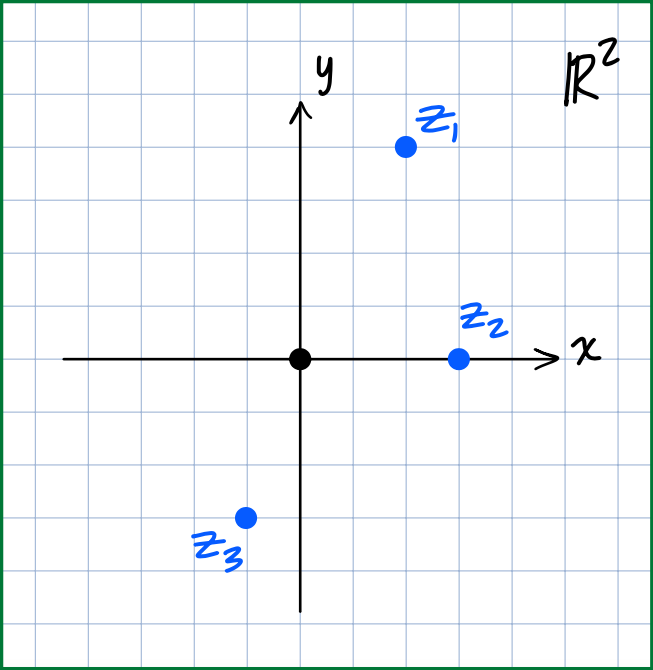
\includegraphics[width=0.3\linewidth]{complexplane}\hspace{4cm} 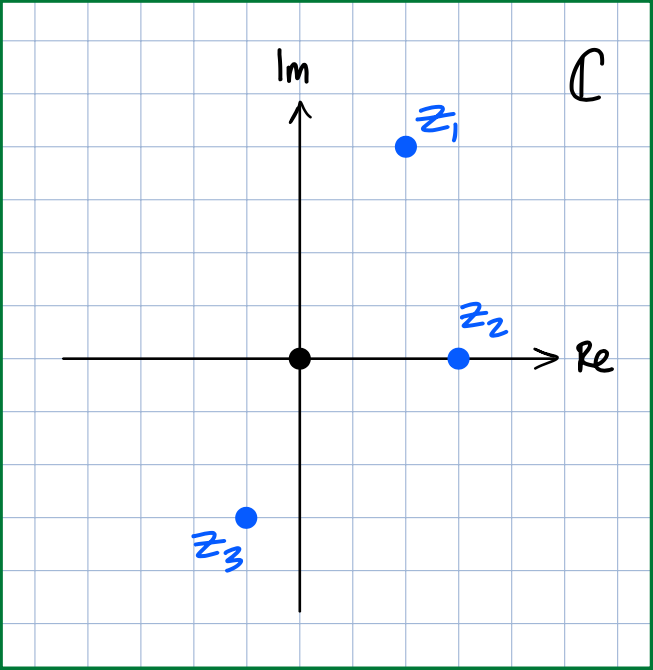
\includegraphics[width=0.3\linewidth]{complexplaneupdated}
\end{center}

\p Note that a point $z\in\COMPLEX$ lies on the $x$-axis if and only if it is real, and lies on the $y$-axis exactly when it is purely imaginary.  On the right, labels are updated accordingly.  $\COMPLEX = \REAL^{2}$ illustrated in this manner is referred to as the \DEF{complex plane}.
\vsp

\p A complex number $z = a + bi$ may also be geometrically represented as an arrow pointing from the origin to the point $(a,b)$ in $\REAL^{2}$, shown on the left.
\vsp

\begin{center}
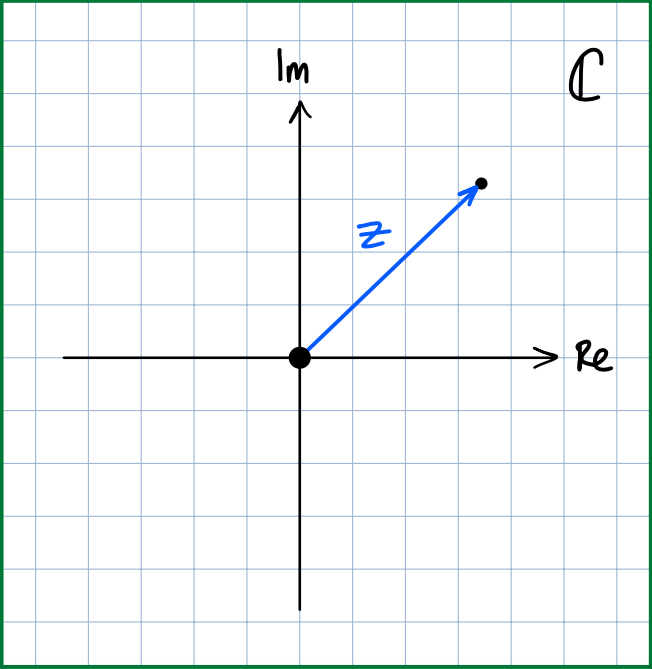
\includegraphics[width=0.3\linewidth]{geometriccomplex}\hspace{4cm} 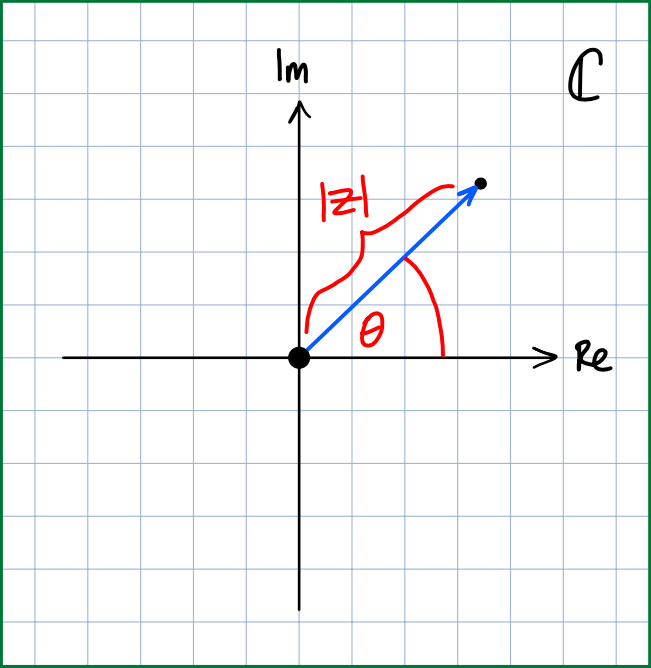
\includegraphics[width=0.3\linewidth]{geometriccomplexlabelled}
\end{center}

\p Any such arrow has length given by the complex modulus of $z$, and forms an angle of inclination, measured counter-clockwise from the positive half of the real axis, shown on the right.

\begin{definition}
An ordered pair $(r,\theta)$ is a polar coordinate representation of $z$ if $r = |z|$ and $\theta$ is the angle of inclination of $z$, measured counter-clockwise from the positive half of the real axis.  In this case $\theta$ is called an \DEF{argument} of $z$.
\end{definition}

\note If $(r,\theta)$ is a polar coordinate representation of a complex number $z$, the Pythagorean Theorem forces real and imaginary parts of $z$ to be given by
\begin{center}
$\RE{z} = r\cos(\theta)$ and $\IM{z} = r\sin(\theta)$.
\end{center}
It follows that $z = r\cos(\theta) + ir\sin(\theta) = r(\cos(\theta) + i\sin(\theta)) = re^{i\theta}$, which is referred to as the \DEF{polar form} of $z$.
\vsp

\observation If $z_{1} = r_{1}e^{i\theta_{1}}$ and $z_{2} = r_{2}e^{i\theta_{2}}$ are written in polar form, then
\begin{center}
$\ds{z_{1}z_{2} = \left(r_{1}e^{i\theta_{1}}\right)\left(r_{2}e^{i\theta_{2}}\right) = (r_{1}r_{2})e^{i\theta_{1} + i\theta_{2}} = r_{1}r_{2}e^{i(\theta_{1} +\theta_{2})}}$
\end{center}
and
\begin{center}
$\ds{z_{1}/z_{2} = \frac{r_{1}e^{i\theta_{1}}}{r_{2}e^{i\theta_{2}}} = \left(\frac{r_{1}}{r_{2}}\right)e^{i\theta_{1} - i\theta_{2}} = \left(\frac{r_{1}}{r_{2}}\right)e^{i(\theta_{1} - \theta_{2})}}$.
\end{center}
\vsp

\p Consequently, to multiply complex numbers in polar form, we \emph{multiply their lengths and add their arguments}.  To divide them, we \emph{divide their lengths, and subtract their arguments}.  This is helpful to make use of when computing powers.  Indeed if $z = re^{i\theta}$ is in polar form and $n\geq 0$, then
\begin{center}
$z^{n} = \left(re^{i\theta}\right)^{n} = r^{n}\left(e^{i\theta}\right)^{n} = r^{n}e^{n(i\theta)} = r^{n}e^{i(n\theta)}$.
\end{center}
\vsp

\p Combining this with Euler's Formula in the special case when $r = 1$, we get the following.
\vsp

\begin{theorem}[DeMoivre's Formula] $(\cos(\theta) + i\sin(\theta))^{n} = \cos(n\theta) + i\sin(n\theta)$
\end{theorem}

\examples
\begin{enumerate}[(a)]
\item Let $z_{1} = 1 + i$ and $z_{2}  = \sqrt{3} - i$.  Find $z_{1}z_{2}$ and $z_{1}/z_{2}$ in polar form.
\item Find $(1 + i)^{16}$.
\end{enumerate}

\subsection{$\ARG{z}$ and $\PARG{z}$}

\p Note that the argument of a complex number is not unique!  For example, in polar form, $1 + i$ may be written as both $\sqrt{2}e^{i(\pi/4)}$ and $\sqrt{2}e^{i(9\pi/4)}$.  So both $\pi/4$ and $9\pi/4$ are arguments for $1 + i$.  More generally, if $\theta$ is an argument for $z\in\COMPLEX$, then so is $\theta + 2\pi k$ for any $k\in \INTEGER$.
\vsp

\notation For any $z\in\COMPLEX$ with argument $\theta$, we may capture all of its arguments with the notation
\begin{center}
$\ARG{z} = \theta + 2\pi k$
\end{center}
where it is understood that $k$ varies over the set of integers.
\vsp

\fact For any $\theta\in\REAL$, there exists a unique $k^{\star}\in\INTEGER$ such that $\theta + 2\pi k^{\star}\in (-\pi, \pi]$.  In this case $\theta + 2\pi k^{\star}$ is called the \DEF{principle argument} of $z$, and is denoted by $\PARG{z}$.
\vsp

\examples
\begin{enumerate}[(a)]
\item For $z = 1 + i$, $\ARG{z} = \pi/4 + 2\pi k$, and $\PARG{z} = \pi/4$.
\item $\PARG{e^{i(5\pi/3)}} = -2\pi/3$.
\end{enumerate}

\begin{exercise} is $Arg(z_1z_2) = Arg(z_1) + Arg(z_2)$?
\end{exercise}

\subsection{Roots of Unity}

\p So far, positive and negative exponents have been defined for complex numbers, but what about rational exponents?  In the case of real numbers, we define
\begin{center}
$x^{m/n} = \sqrt[n]{x^{m}} = \left(\sqrt[n]{x}\right)^{m}$,
\end{center}
whenever $\GCD{m,n} = 1$ and either $x\geq 0$ or $n$ is odd.
\vsp

\p But this takes advantage $n$th roots, which have not yet been defined for complex numbers.  This notion must first be extended to $\COMPLEX$.  But this is no simple matter, since in $\REAL$ for example, there are two fourth roots of $1$: namely $1$ and $-1$.  This is traditionally resolved by defining $\sqrt[4]{1}$ to be the \emph{positive} fourth root of $1$, and then using the notation $\pm \sqrt[4]{1}$ to describe both of the fourth roots of $1$.
\vsp

\p But in $\COMPLEX$, $1$, $-1$, $i$ and $-i$ are \emph{all} fourth roots of $1$!  A new method must be developed to capture all of these roots.
\vsp

\begin{definition}
Let $n\geq 1$.  A complex number $\zeta$ is said to be an \DEF{$n$th root of unity} if $\zeta^{n} = 1$.
\end{definition}

\example The fourth roots of unity are the complex numbers $1, -1, i$, and $i$.
\vsp

\p For a general $n\geq 1$, it is easier to construct an $n$th root of unity when polar form is considered.
\vsp

\remarks
\begin{enumerate}[(1)]
\item For any integer $n\geq 1$, if $\zeta = e^{i(2\pi/n)}$, it may be seen that
\begin{center}
$\zeta^{n} = \left(e^{i(2\pi/n)}\right)^{n} = e^{n[i(2\pi/n)]} = e^{i(2\pi)} = 1$.
\end{center}
\p Hence $\zeta = e^{i(2\pi/n)} = \cos(2\pi/n) + i\sin(2\pi/n)$ is an $n$th root of unity.
\item For any $k\in\INTEGER$, $\zeta^{k}$ is also an $n$th root of unity.  Indeed we may compute
\begin{center}
$\left(\zeta^{k}\right)^{n} = \left(\zeta^{n}\right)^{k} = 1^{k} = 1$.
\end{center}
\item The $n$ distinct $n$th roots of unity are given by $\zeta^{k} = e^{i(2\pi k/n)}$, where $k\in\INTEGER$ with $0\leq k < n$.
\end{enumerate}

\example Find all of the eighth roots of unity.

\begin{definition} Let $n\geq 1$.  A complex number $\omega\in\COMPLEX$ is a \DEF{primitive $n$th root of unity} if $\omega^{n} = 1$ and $\omega^{k}\neq 1$ whenever $0 < k < n$.
\end{definition}

\p classify all $n$th roots of unity: if $\omega$ is primitive, then the set of $n$th roots of unity is given by $\SET{\omega^{k}:k=0,1,\dots,n-1}$

\p when is $\omega^{k}$ primitive? when $\GCD{n,k} = 1$

\p solutions to $z^{n} = z_{0} = re^{i\theta}$ are found by taking $r^{1/n}e^{i(\theta/n)}$ and multiplying it by all the different roots of unity

\p -quadratic formula
\end{document}

